\section{Modeling}\label{sec:modeling}
In order to model the Jao Gap we evolve two extremly finely sampled mass grid
of models. One of these grids uses the OPAL high-temperature opacity tables
while the other uses the OPLIB tables (Figure \ref{fig:PunchIn}). Each grid
evolves a model every 0.00025 $M_{\odot}$ from 0.2 to 0.4 $M_{\odot}$ and every
0.005 $M_{\odot}$ from 0.4 to 0.8 $M_{\odot}$. All models in both grids use a
GS98 solar composition, the (1, 101, 0) \texttt{Free\_EOS} (version
{\color{red}2.7}) configuration, and 1000 year old pre-main sequence polytropic
models, with polytropic index 1.5, as their initial conditions.

Because in this work we are just interested in the location shift of the gap as
the opacity source varies, we do not model variations in composition.
\citet{Mansfield2021,Jao2020,Feiden2021} all look at the effect composition has
on Jao Gap location. They find that as population metallicity increase so to
does the mass range and consequently the magnitude of the Gap. From an extremely
low metallicity population (Z=0.001) to a population with a more solar like
metallicity this shift in mass range can be up to 0.05 M$_{\odot}$
\citep{Mansfield2021}.

\begin{figure}
	\centering
	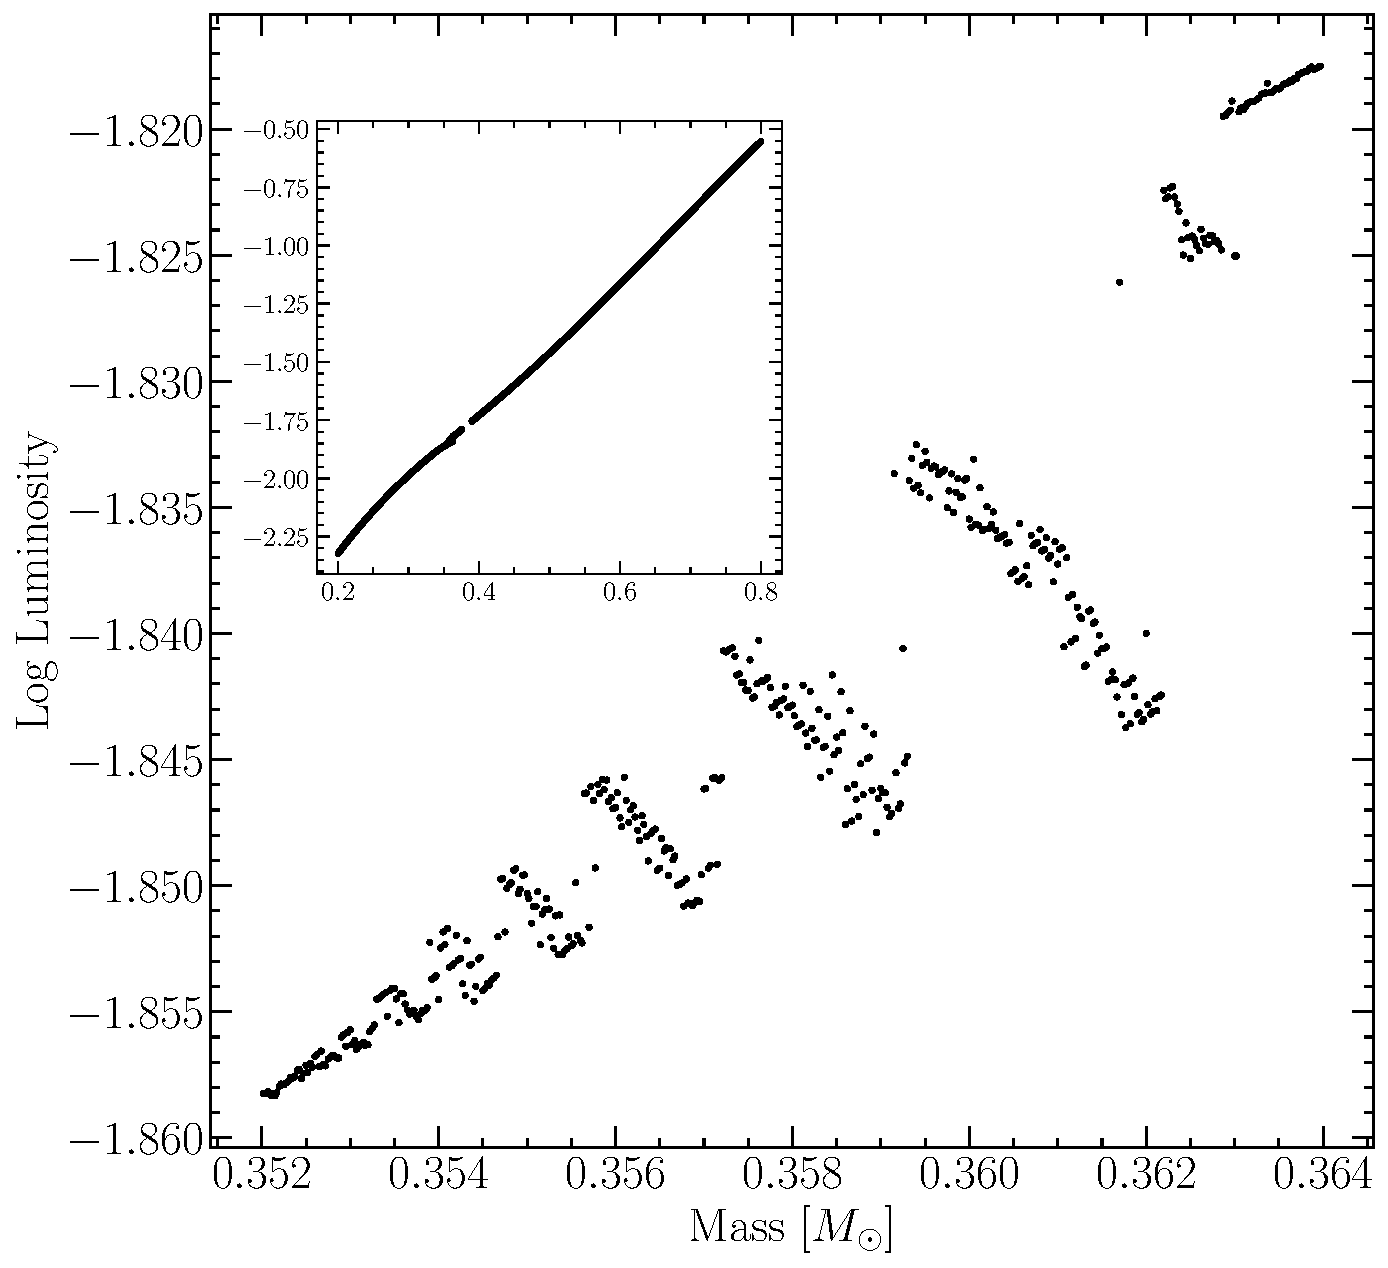
\includegraphics[width=0.45\textwidth]{src/figures/NotebookFigs/OPALPunchIn.pdf}
	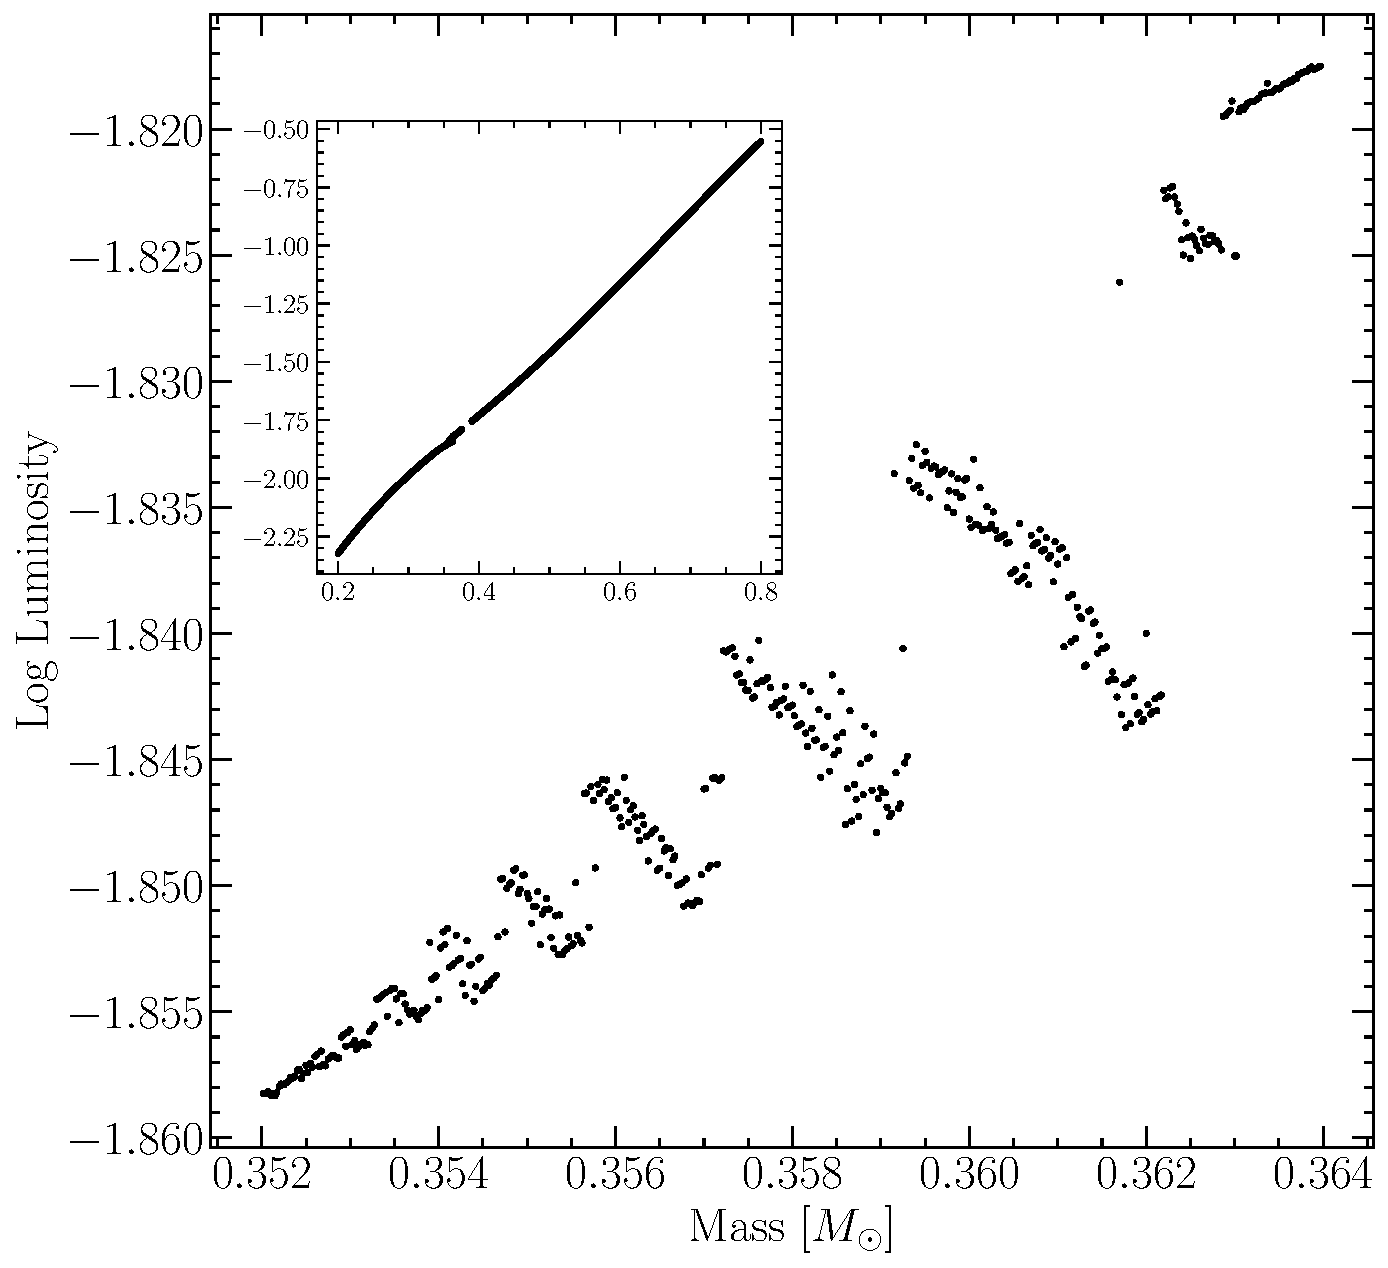
\includegraphics[width=0.45\textwidth]{src/figures/NotebookFigs/OPALPunchIn.pdf}
	\caption{Mass-luminosity relation for models evolved using OPAL opacity
	tables (top) and those evolved using OPLIB opacity tables (bottom)
	{\color{red}[UPDATE OPLIB FIG WHEN MODELS DONE]}. Note the lower mass range
	of the OPLIB Gap.}
	\label{fig:PunchIn}
		
\end{figure}

\subsection{Population Synthethis}
In order to compare the gap to observations we use in house population
synthesis code. Our population synthesis code first uses inverse CDF sampling
to build a distribution of target masses from some initial mass function (IMF).
Specifically we use the \citet{Sollima2019} IMF where, for masses 0.25
$M_{\odot} < M < 1 M_{\odot}$, $\alpha=-1.34\pm0.07$. The model nearest in mass
to the samples mass above and the nearest model below are then selected from
the evolved model database. The surface gravity, luminosity, and effective
temperature of the sample are estimated from a linear interpolation between the
upper and lower bounding models. $T_{eff}$, $g$, and $log(L)$ are transformed
into Gaia G, BP, and RP magnitudes using the bolometric corrections provided by
the Gaia Collaboration, specifically \texttt{fehp000.UBVRIplus}
{\color{red}[CITATION]} {\color{red}[How to cite Aarons code]}. Next, we
introduce observationally informed photometric and astrometric uncertainties
into our population.

We select the Gaia Catalogue of Nearby Stars (GCNS) {\color{red}[CITATION]} to
empirically calibrate uncertainty relations. A function with the form of
Equation \ref{eqn:plxCalib} is fit to parallax uncertainty vs. G magnitude.
Additionally, a function of the form of Equation \ref{eqn:MagCalib} is fit to
to i$^{\text{th}}$ (G, BP, RP) magnitude uncertainty vs. i$^{\text{th}}$
magnitude.

\begin{align}\label{eqn:plxCalib}
	\sigma_{plx}(M_{g}) = ae^{bM_{g}}+c
\end{align}
\begin{align}\label{eqn:MagCalib}
	\sigma_{i}(M_{i}) = ae^{M_{i}-b}+c
\end{align}

\begin{figure}
	\centering
	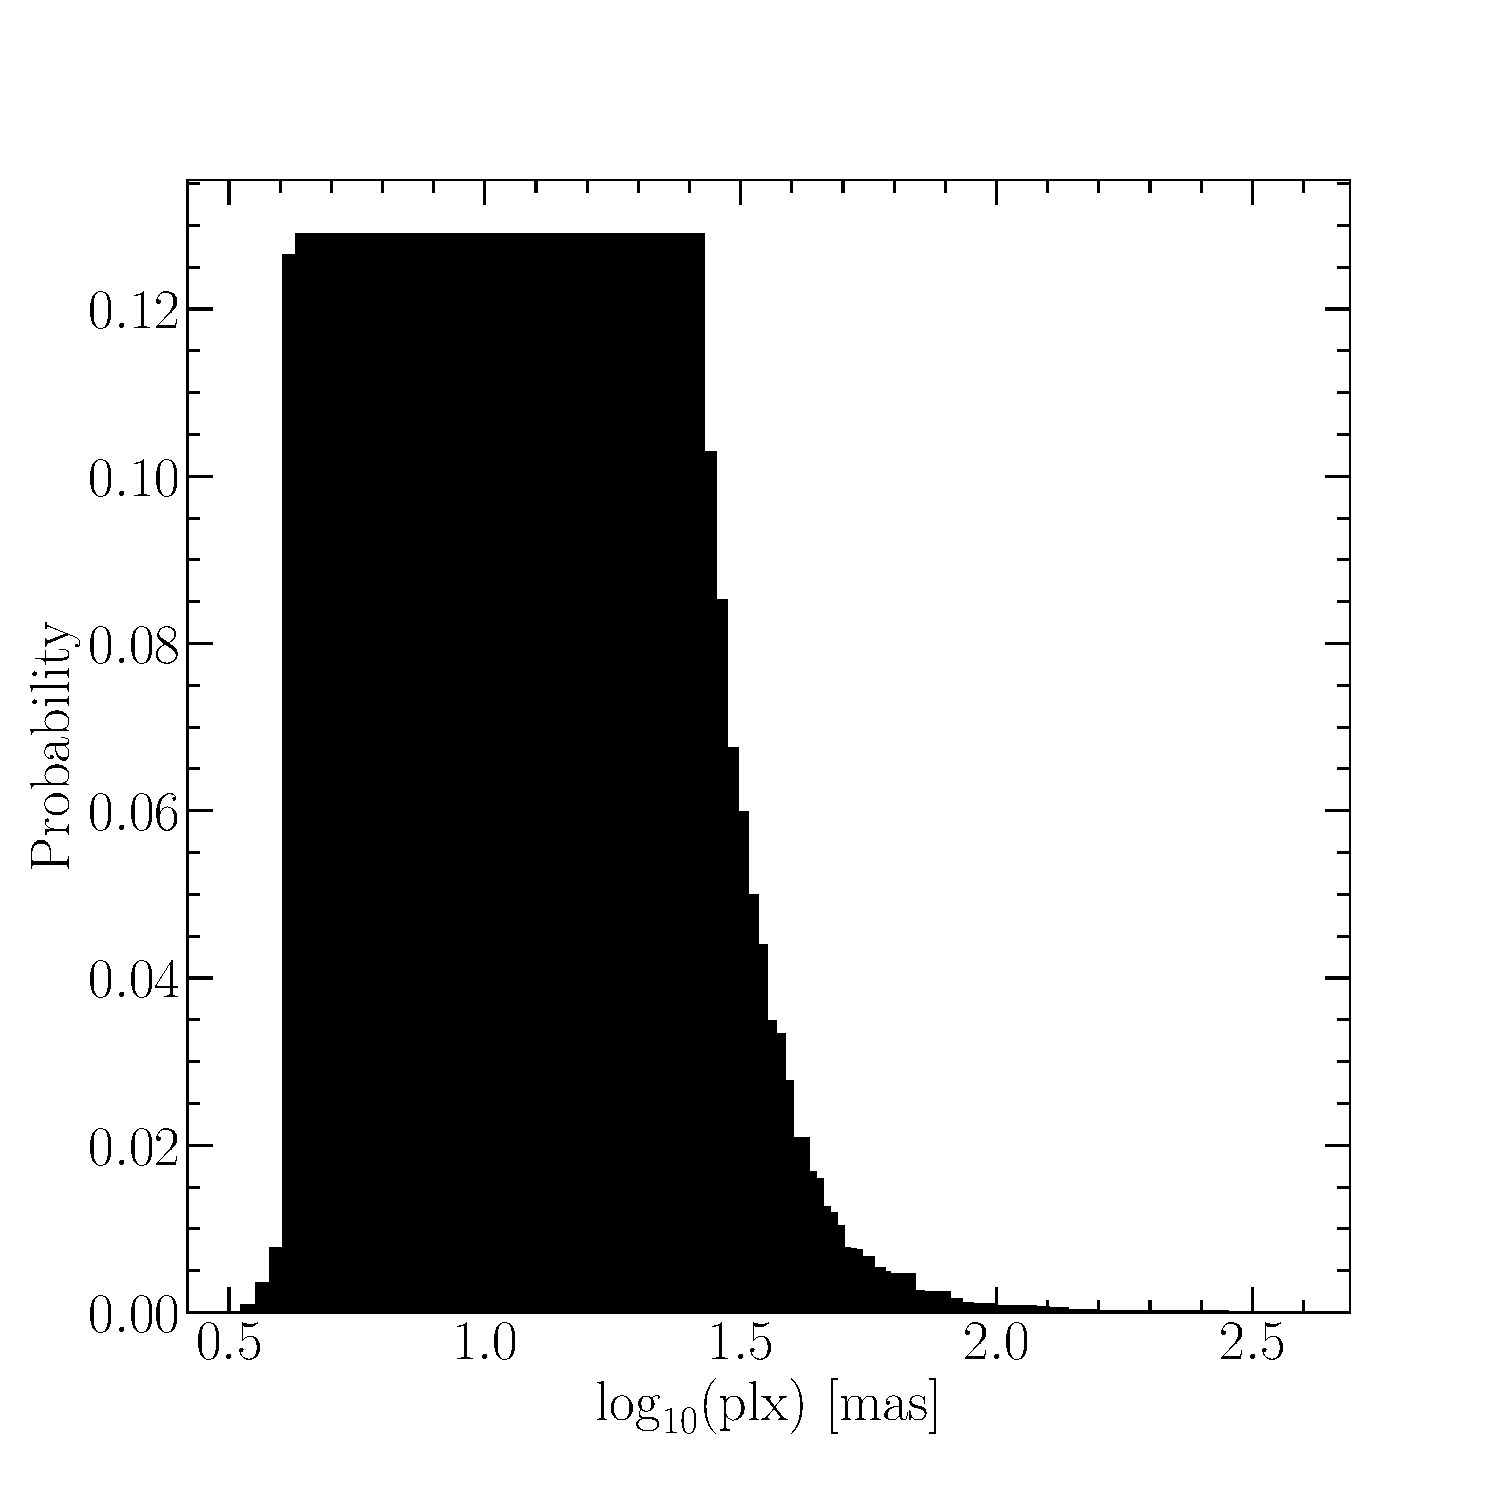
\includegraphics[width=0.45\textwidth]{src/figures/NotebookFigs/pdist.pdf}
	\caption{Probability distribution sampled when assigning true parallaxs to
	synthetic stars. This distribution is built from the GCNS.}
	\label{fig:pdist}
\end{figure}

Each of these functions estimates the uncertainty of some quantity at a given
magnitude. Moreover, for each sampled in the synthetic population we sample a
parallax from the distribution in the GCNS (Figure \ref{fig:pdist}), referred
to as the ``true parallax''. A parallax uncertainty is calculated based on the
empirically calibrated parallax uncertainty and G-magnitude relation along with
the synthetic stars G-magnitude (hereafter the ``true G magnitude) and the
results of the fitting described in the previous paragraph. This uncertainty
is then, with equal weighting, either be added or subtracted from the true
Parallax, yielding an ``observed parallax''.

The true parallax is used to convert the true i$^{\text{th}}$ magnitude to an
apparent i$^{\text{th}}$ magnitude and the observed parallax is used to convert
the apparent i$^{\text{th}}$ magnitude into an observed i$^{\text{th}}$
magnitude. Finally, each observed magnitude is summed with an estimated
photometric uncertainty for that magnitude based on the fit of the
i$^{\text{th}}$ magnitude to the uncertainty in the i$^{\text{th}}$ magnitude.

To summarize the process that each synthetic star will go through
\begin{enumerate}
	\item Sample from a \citet{Sollima2019} IMF to determine synthetic star mass
	\item Find the closest model above and below the synthetic star, linerally
		interpolate model parameters to the synthetic star mass.
	\item Convert synthetic star $g$, $T_{eff}$, and $Log(L)$ to Gaia G, BP,
		and RP colors.
	\item Sample from the GCNS to assign synthetic star a ``true'' parallax.
	\item Evaluate the empirical calibration given in Equation
		\ref{eqn:plxCalib} to find an associated parallax uncertainty and
		adjust the true parallax by this value resulting in an observed
		parallax.
	\item Use the true parallax to find an apparent magnitude for each filter.
	\item Use the observed parallax and the apparent magnitude to find an
		observed magnitude
	\item Evaluate the empirical calibration given in Equation
		\ref{eqn:MagCalib} to give a magnitude uncertainty scale in each band.
	\item Adjust each magnitude by some amount sampled from a normal
		distribution with a standard deviation of the magnitude uncertainty
		scale.
\end{enumerate}

This method then incorporates both photometric and astrometric uncertainties
into our population synthesis. An example seven Gyr old synthetic populations
using OPAL and OPLIB opacities are given in Figure
\ref{fig:PopSynthCompareBasic}.

\begin{figure*}
	\centering
	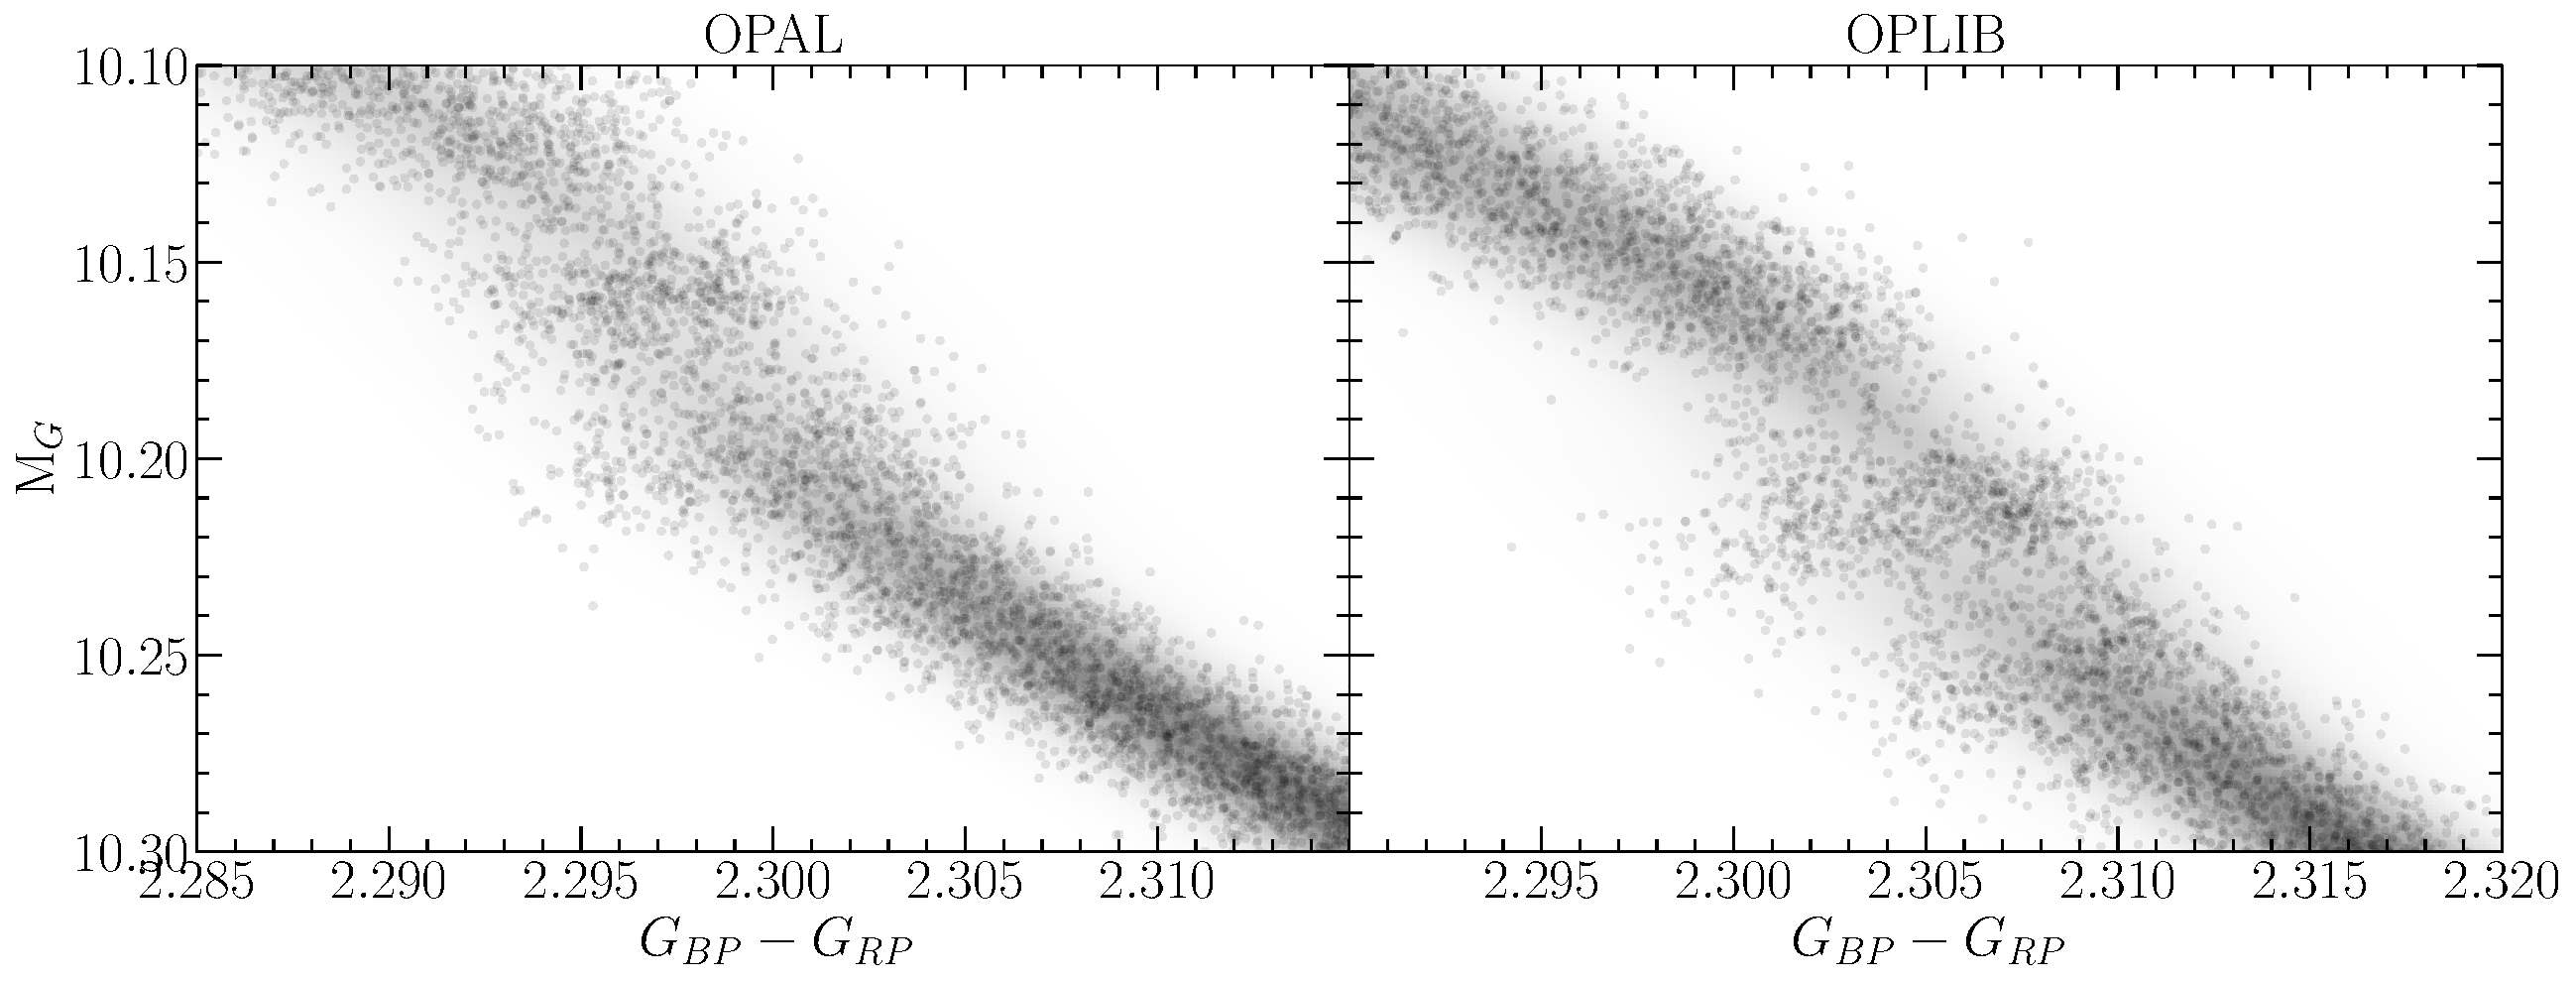
\includegraphics[width=0.85\textwidth]{src/figures/NotebookFigs/OPALOPLIB_popsynth_compare.pdf}
	\caption{Population synthetis resulst for models evolved with OPAL (left)
	and models evolved with OPLIB (right). A gaussian kernel-density-estimate
	has been overlayed to better highlight the density variations. {\color{red}
	[THIS IS A PLACEHOLDER FIGURE]}}
	\label{fig:PopSynthCompareBasic}
\end{figure*}
